% https://www.latex4technics.com/?note=5rc
% https://tex.stackexchange.com/a/241153/173708
\documentclass[tikz]{standalone}

\begin{document}
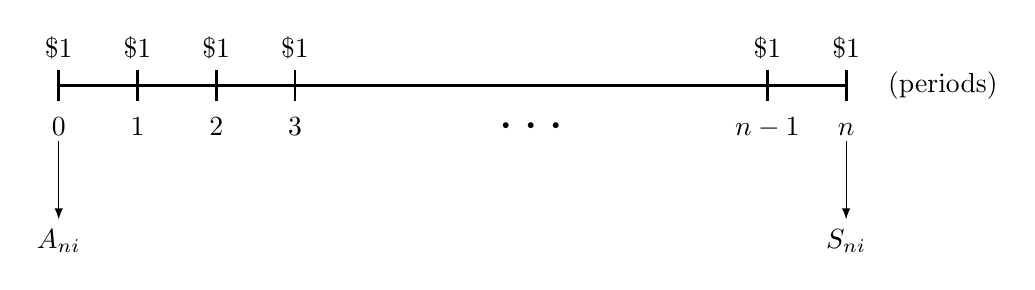
\begin{tikzpicture}
  \draw[line width=1pt] (0,0) -- node[below=1mm,pos=0.6,scale=2] {$\cdots$} (10,0)node[right=4mm]{(periods)};
  \foreach \x/\y in {0/0,1/1,2/2,3/3,9/$n-1$,10/$n$}{
    \draw[line width=1pt] (\x,-2mm)node[below](\x){\strut\y} -- (\x,2mm)node[above]{$\$ 1$};
    }
    \draw[-latex] (0,-7mm) -- +(0,-10mm)node[below]{$A_{ni}$};
    \draw[-latex] (10,-7mm) -- +(0,-10mm)node[below]{$S_{ni}$};
\end{tikzpicture}
\end{document}